\chapter{BCD译码器}

\section{第一步：解决什么问题}

计算机内部使用二进制运算，但人类需要看到十进制数字。

\textbf{问题}：FPGA内部计算结果是4位二进制（0000到1111），如何在7段数码管上显示为人类可读的十进制数字（0到9）？

\textbf{方案}：将4位BCD码（Binary-Coded Decimal）转换为7段数码管的驱动信号。

BCD码：用4位二进制数表示一个十进制数字。

\begin{itemize}
  \item 0 $\to$ 0000
  \item 1 $\to$ 0001
  \item 2 $\to$ 0010
  \item ...
  \item 9 $\to$ 1001
\end{itemize}

注意：1010到1111（10到15）在BCD中是非法的，不应出现。

\section{第二步：输入输出关系}

\begin{itemize}
  \item \textbf{输入}：$A_3, A_2, A_1, A_0$（4位BCD码，表示0-9）
  \item \textbf{输出}：$a, b, c, d, e, f, g$（7段，每一段控制数码管的一段LED）
\end{itemize}

7段数码管的段命名：

\begin{center}
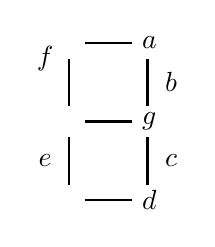
\begin{tikzpicture}[scale=1.0]
  % 7-segment display with segment labels
  \draw[thick] (0,2) -- (0.6,2) node[right] {$a$};  % top
  \draw[thick] (0.8,1.2) -- (0.8,1.8);              % top-right: b
  \draw[thick] (0.8,0.2) -- (0.8,0.8);              % bottom-right: c
  \draw[thick] (0,0) -- (0.6,0) node[right] {$d$};  % bottom
  \draw[thick] (-0.2,0.2) -- (-0.2,0.8);            % bottom-left: e
  \draw[thick] (-0.2,1.2) -- (-0.2,1.8);            % top-left: f
  \draw[thick] (0,1) -- (0.6,1) node[right] {$g$};  % middle
  \node at (-0.5,1.8) {$f$};
  \node at (1.1,1.5) {$b$};
  \node at (-0.5,0.5) {$e$};
  \node at (1.1,0.5) {$c$};
\end{tikzpicture}
\end{center}

\section{第三步：真值表}

\begin{center}
\small
\begin{tabular}{|c|c|c|c||c|c|c|c|c|c|c||c|}
\hline
$A_3$ & $A_2$ & $A_1$ & $A_0$ & $a$ & $b$ & $c$ & $d$ & $e$ & $f$ & $g$ & 显示 \\
\hline
0 & 0 & 0 & 0 & 1 & 1 & 1 & 1 & 1 & 1 & 0 & 0 \\
0 & 0 & 0 & 1 & 0 & 1 & 1 & 0 & 0 & 0 & 0 & 1 \\
0 & 0 & 1 & 0 & 1 & 1 & 0 & 1 & 1 & 0 & 1 & 2 \\
0 & 0 & 1 & 1 & 1 & 1 & 1 & 1 & 0 & 0 & 1 & 3 \\
0 & 1 & 0 & 0 & 0 & 1 & 1 & 0 & 0 & 1 & 1 & 4 \\
0 & 1 & 0 & 1 & 1 & 0 & 1 & 1 & 0 & 1 & 1 & 5 \\
0 & 1 & 1 & 0 & 1 & 0 & 1 & 1 & 1 & 1 & 1 & 6 \\
0 & 1 & 1 & 1 & 1 & 1 & 1 & 0 & 0 & 0 & 0 & 7 \\
1 & 0 & 0 & 0 & 1 & 1 & 1 & 1 & 1 & 1 & 1 & 8 \\
1 & 0 & 0 & 1 & 1 & 1 & 1 & 1 & 0 & 1 & 1 & 9 \\
\hline
\end{tabular}
\end{center}

对于1010到1111（10-15），输出通常全部熄灭（全0）或显示特定模式（取决于设计）。

\section{第四步：逻辑推导}

每一段都是一个4变量组合逻辑函数。以$a$段为例：

$a = 1$ 当输入为：0(0000), 2(0010), 3(0011), 5(0101), 6(0110), 7(0111), 8(1000), 9(1001)

即：$a = \sum m(0,2,3,5,6,7,8,9)$

卡诺图化简后（此处省略卡诺图步骤，这是我们有意跳过的部分），得到：

\begin{align}
  a &= A_3 + A_1 + \overline{A_2}\cdot\overline{A_0} + A_2\cdot A_0 \\
  b &= \overline{A_2} + \overline{A_1}\cdot\overline{A_0} + A_1\cdot A_0 \\
  c &= \overline{A_1} + A_0 + A_2 \\
  d &= \overline{A_2}\cdot\overline{A_0} + A_1\cdot\overline{A_0} + \overline{A_2}\cdot A_1 + A_2\cdot\overline{A_1}\cdot A_0 \\
  e &= \overline{A_2}\cdot\overline{A_0} + A_1\cdot\overline{A_0} \\
  f &= A_3 + \overline{A_1}\cdot\overline{A_0} + A_2\cdot\overline{A_1} + A_2\cdot\overline{A_0} \\
  g &= A_3 + \overline{A_2}\cdot A_1 + A_1\cdot\overline{A_0} + A_2\cdot\overline{A_1}
\end{align}

但在考试中，\textbf{你不会也不需要手算这些表达式}。考试更可能考的是理解BCD译码器的功能和使用方法。

\section{第五步：结构化设计}

BCD-7段译码器 = 7个4变量组合逻辑函数，每个函数通过ROM/查找表实现：

\begin{center}
\begin{tikzpicture}
  \node[draw, minimum width=3cm, minimum height=4cm] (rom) at (0,0) {ROM/查找表};
  \node (A) at (-3,1) {$A_{3:0}$};
  \node (seg) at (3,1) {$a,b,c,d,e,f,g$};
  \draw[->] (A) -- (rom.west |- A);
  \draw[->] (rom.east |- seg) -- (seg);
  \node at (0,-3) {输入：4位BCD → 查表 → 输出：7段控制信号};
\end{tikzpicture}
\end{center}

\section{第六步：为什么这样设计}

\begin{enumerate}
  \item \textbf{为什么用查找表而非单独的门电路？}

  7段译码器涉及7个4变量函数。如果每个都用门电路实现，需要大量AND门和OR门。使用ROM（16×7 = 112 bits）更简洁，这也是FPGA中LUT（查找表）的实际实现方式。

  \item \textbf{为什么1010-1111是非法输入？}

  BCD码的定义：4位二进制只使用前10个编码（0000-1001）。后6个编码（1010-1111）不表示任何十进制数字，是非法BCD码。好的设计应该对所有输入都定义行为（全部熄灭或显示异常标记）。

  \item \textbf{与普通3-8译码器的本质区别？}

  3-8译码器：每个输出是\textbf{一个}最小项（3输入AND）
  BCD-7段译码器：每个输出是\textbf{多个}最小项之和（4输入的组合逻辑函数）

  所以BCD-7段译码器本质上是7个独立的组合逻辑函数。
\end{enumerate}

\section{第七步：考试常见变式}

\begin{enumerate}
  \item \textbf{变式1：多位BCD显示}

  多个BCD译码器 + 多个7段数码管，实现多位数显示。通常配合动态扫描技术（快速轮流点亮各数码管，利用人眼视觉暂留）。

  \item \textbf{变式2：带锁存功能的BCD译码器}

  输入锁存：在LE（Latch Enable）信号控制下锁存当前BCD输入，数码管保持显示不变。这在需要稳定显示时非常有用。

  \item \textbf{变式3：共阳极 vs 共阴极数码管}

  共阳极：所有LED阳极接一起（接VCC），段驱动需要低电平点亮（输出0 = 亮）
  共阴极：所有LED阴极接一起（接GND），段驱动需要高电平点亮（输出1 = 亮）

  两种类型的输出值恰好互为反码。

  \item \textbf{变式4：计数 + 显示系统}

  这是考试常见综合题：计数器产生BCD码 $\to$ BCD译码器 $\to$ 7段数码管显示。考察对整个数字系统流程的理解。

  \item \textbf{变式5：16进制显示译码器}

  输入0-15（全4位二进制），输出0-9 + A-F。比BCD译码器多6个有效输入状态。
\end{enumerate}

\section{第八步：VHDL实现}

\begin{lstlisting}[caption={BCD-7段译码器（case版本）}]
library ieee;
use ieee.std_logic_1164.all;

entity bcd_7seg is
  port (
    bcd : in  std_logic_vector(3 downto 0);
    seg : out std_logic_vector(6 downto 0)  -- a,b,c,d,e,f,g
  );
end bcd_7seg;

architecture behavioral of bcd_7seg is
begin
  process(bcd)
  begin
    case bcd is
      when "0000" => seg <= "1111110";  -- 0
      when "0001" => seg <= "0110000";  -- 1
      when "0010" => seg <= "1101101";  -- 2
      when "0011" => seg <= "1111001";  -- 3
      when "0100" => seg <= "0110011";  -- 4
      when "0101" => seg <= "1011011";  -- 5
      when "0110" => seg <= "1011111";  -- 6
      when "0111" => seg <= "1110000";  -- 7
      when "1000" => seg <= "1111111";  -- 8
      when "1001" => seg <= "1111011";  -- 9
      when others => seg <= "0000000";  -- 全灭
    end case;
  end process;
end behavioral;
\end{lstlisting}

\section{第九步：Testbench验证}

\begin{lstlisting}[caption={BCD-7段译码器Testbench}]
library ieee;
use ieee.std_logic_1164.all;

entity bcd_7seg_tb is
end bcd_7seg_tb;

architecture test of bcd_7seg_tb is
  signal bcd : std_logic_vector(3 downto 0);
  signal seg : std_logic_vector(6 downto 0);

  component bcd_7seg is
    port (
      bcd : in  std_logic_vector(3 downto 0);
      seg : out std_logic_vector(6 downto 0)
    );
  end component;
begin
  uut: bcd_7seg port map (bcd, seg);

  stimulus: process
  begin
    for i in 0 to 15 loop
      bcd <= std_logic_vector(to_unsigned(i, 4));
      wait for 10 ns;
    end loop;
    wait;
  end process;
end test;
\end{lstlisting}

\section{第十步：如何快速解题}

\begin{examtip}[BCD译码器快速解题法]
\begin{enumerate}
  \item \textbf{case实现是标准答案}：在VHDL中用case列举10个有效输入，不需要推导门级表达式
  \item \textbf{注意有效电平}：共阳极（0亮）vs共阴极（1亮），输出值互为反码
  \item \textbf{非法输入处理}：1010-1111用when others，全灭或显示特定标记
  \item \textbf{综合题}：计数器+译码器+数码管 = 经典考试题
\end{enumerate}
\end{examtip}

\section{变式详解}
\chapter{BCD译码器——5大变式详解}

\section{变式1：多位BCD动态扫描显示}

\begin{detailbox}[完整教学]
\textbf{【问题】}4位数码管需要4个BCD-7段译码器吗？如果每个译码器单独驱动→需要4×7=28个IO口。

\textbf{【方案】}动态扫描：1个译码器驱动所有数码管的段，快速轮流点亮各数码管（>50Hz），利用人眼视觉暂留。

\textbf{【电路】}
计数器→2-4译码器→轮流选通4个数码管的共阴/共阳极。BCD译码器输出段码到所有数码管。

\textbf{【VHDL核心逻辑】}
\begin{lstlisting}
process(clk)  -- 扫描时钟(通常>200Hz)
begin
  if rising_edge(clk) then
    scan_cnt <= scan_cnt + 1;
    case scan_cnt is
      when "00" => digit_sel <= "0001"; seg_data <= digit0;
      when "01" => digit_sel <= "0010"; seg_data <= digit1;
      when "10" => digit_sel <= "0100"; seg_data <= digit2;
      when "11" => digit_sel <= "1000"; seg_data <= digit3;
    end case;
  end if;
end process;
\end{lstlisting}

\textbf{【常见考题】}设计4位动态扫描显示电路。
\end{detailbox}


\section{变式2：带锁存的BCD译码器}

\begin{detailbox}[完整教学]
\textbf{【问题】}BCD译码器输入随时钟快速变化→数码管闪烁。需要"定格"显示。

\textbf{【方案】}在译码器前加寄存器。LE=1时锁存当前BCD值，LE=0时保持上次锁存值不变。

\textbf{【VHDL】}
\begin{lstlisting}
process(clk)
begin
  if rising_edge(clk) then
    if LE = '1' then
      latched_bcd <= bcd_input;  -- 锁存
    end if;
  end if;
end process;
seg <= bcd_to_7seg(latched_bcd);  -- 译码锁存后的值
\end{lstlisting}

\textbf{【设计思想】}锁存=寄存器=1个时钟沿保存数据。本质=在数据通路上插入一级寄存器。
\end{detailbox}


\section{变式3：共阳极 vs 共阴极数码管}

\begin{detailbox}[完整教学]
\textbf{【共阳极】}所有LED阳极接VCC。段驱动需低电平(0)点亮LED。seg='0'=亮。
\textbf{【共阴极】}所有LED阴极接GND。段驱动需高电平(1)点亮LED。seg='1'=亮。

\textbf{【输出值关系】}$seg_{\text{共阳}} = \text{not } seg_{\text{共阴}}$（互为反码）

\textbf{【VHDL适配】}
\begin{lstlisting}
-- 共阴极(1亮)
when "0000" => seg <= "1111110";  -- 0
-- 共阳极(0亮)
when "0000" => seg <= "0000001";  -- 0(反码)
\end{lstlisting}

\textbf{【考试陷阱】}题目未明确说明共阴/共阳时，看段码值判断：1111110(共阴0) vs 0000001(共阳0)。
\end{detailbox}


\section{变式4：计数器+译码器+数码管——综合题}

\begin{detailbox}[完整教学]
\textbf{【经典考题】}设计0-9计数器+BCD-7段译码器+数码管显示。

\textbf{【完整VHDL】}
\begin{lstlisting}
entity counter_display is
  port (clk, rst_n : in std_logic;
        seg : out std_logic_vector(6 downto 0));
end counter_display;

architecture rtl of counter_display is
  signal cnt : std_logic_vector(3 downto 0);
  function bcd7seg(bcd : std_logic_vector(3 downto 0))
    return std_logic_vector is
  begin
    case bcd is
      when "0000" => return "1111110";
      when "0001" => return "0110000";
      when "0010" => return "1101101";
      when "0011" => return "1111001";
      when "0100" => return "0110011";
      when "0101" => return "1011011";
      when "0110" => return "1011111";
      when "0111" => return "1110000";
      when "1000" => return "1111111";
      when "1001" => return "1111011";
      when others => return "0000000";
    end case;
  end function;
begin
  process(clk, rst_n)
  begin
    if rst_n='0' then cnt <= "0000";
    elsif rising_edge(clk) then
      if cnt = "1001" then cnt <= "0000";
      else cnt <= cnt + 1;
      end if;
    end if;
  end process;
  seg <= bcd7seg(cnt);
end rtl;
\end{lstlisting}

\textbf{【考点】}两个模块整合：计数器+译码器。
\end{detailbox}


\section{变式5：16进制显示译码器（0-F）}

\begin{detailbox}[完整教学]
\textbf{【问题】}BCD译码器只显示0-9。如何显示0-F（全4位二进制）？

\textbf{【方案】}扩展case覆盖1010-1111，定义A-F的段码。

\begin{lstlisting}
-- 扩展BCD译码器支持0-F
when "1010" => return "1110111";  -- A
when "1011" => return "0011111";  -- b
when "1100" => return "1001110";  -- C
when "1101" => return "0111101";  -- d
when "1110" => return "1001111";  -- E
when "1111" => return "1000111";  -- F
\end{lstlisting}

\textbf{【考试】}有时问A-F的段码值，需要记住典型表示法。
\end{detailbox}
